\documentclass{article}

\usepackage[hyphens]{url}
\usepackage[hidelinks]{hyperref}

\usepackage[fontsize=12]{fontsize}
% \usepackage{fullpage}
\usepackage[a4paper]{geometry}
\geometry{left=2.5 cm,right=2.5 cm, top=1.5 cm, bottom=2 cm}
\usepackage{graphicx}
\usepackage{placeins}
\usepackage[parfill]{parskip}

\usepackage{caption}
\usepackage{subcaption}
\usepackage{natbib}
\bibliographystyle{abbrvnat}
\usepackage{titlesec}
\newcommand{\dd}{$\Delta\Delta$}
\titleformat*{\section}{\large\bfseries}
% \renewcommand{\baselinestretch}{2}
% \author{Jeremy Ocampo}
% \title{\textbf{Prediction of single point protein mutations stability changes.}}
% \date{}
\begin{document}
\vspace{-1cm}
\begin{center}
    \Large{\textbf{Prediction of single point protein mutation stability changes with the Mega-scale dataset.}} \\
    \vspace{0.5cm}
    Jeremy Ocampo
\end{center}

\section{Problem analysis}
Understanding the mechanisms in protein stability is important, since even a single amino acid mutation can be the cause of a disease. The effect of a mutation on a protein is usually assessed by the difference of the Gibbs free energy between the mutated and wild-type form protein, denoted $\Delta\Delta$G (denoted \texttt{score} in the dataset).

\textbf{Exploratory data analysis.} We should explore the dataset first in order to find which variables have a high predictive power of $\Delta\Delta$G. There are 310 different wildtype proteins (\texttt{pdbid}) which isn't much, this means it would be harder for machine learning models to generalize to ``unseen" protein structures. But there are 340k data points which should be enough for a neural network to perform well given we design it carefully. We also make a number of plots with descriptions, in Figure \ref{fig:lenpos} we show the dependance of \dd G with protein length and mutation position. Figure \ref{fig:wildtype} shows the \dd G dependance on the wildtype, and Figure \ref{fig:mutation} shows the dependance on the amino acid mutation.

\begin{figure}[!htb]
    \centering
    \begin{subfigure}[b]{0.45\textwidth}
        \centering
        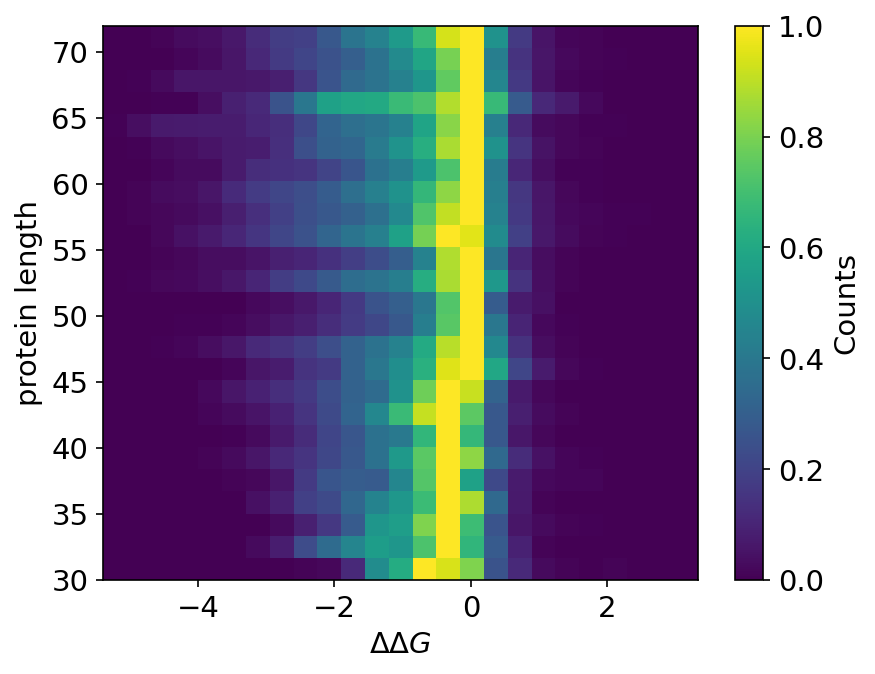
\includegraphics[width=\textwidth]{plots/protein_lengths.png}
        \caption{$\Delta\Delta$G vs protein length}
        \label{fig:lengths}
    \end{subfigure}
    \hfill
    \begin{subfigure}[b]{0.45\textwidth}
        \centering
        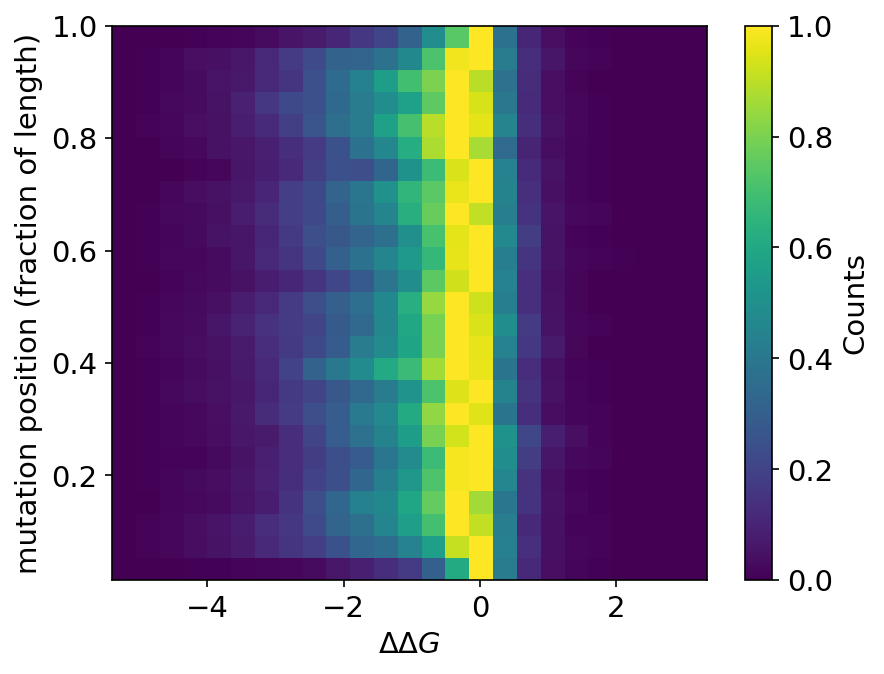
\includegraphics[width=\textwidth]{plots/mutation_position.png}
        \caption{$\Delta\Delta$G vs mutation position}
        \label{fig:position}
    \end{subfigure}
    \caption{2D histograms of $\Delta\Delta$G vs protein length or mutation position (as a fraction of the protein length). For fair comparison at each length, we've normalized each row of the histogram by the max. It seems like there is not much correlation with length, only slightly less energy for lower lengths. Presumably, this is because there are less electrostatic interactions for shorter proteins, but because they can fold in all sorts of ways, there is a spread in \dd G. There's not much correlation with mutation position either, except at the ends of the protein which have mostly no change in \dd G, presumably because there are less atoms and bonds around the ends of the protein.}
    \label{fig:lenpos}
\end{figure}
\FloatBarrier

\begin{figure}[!htb]
    \centering
    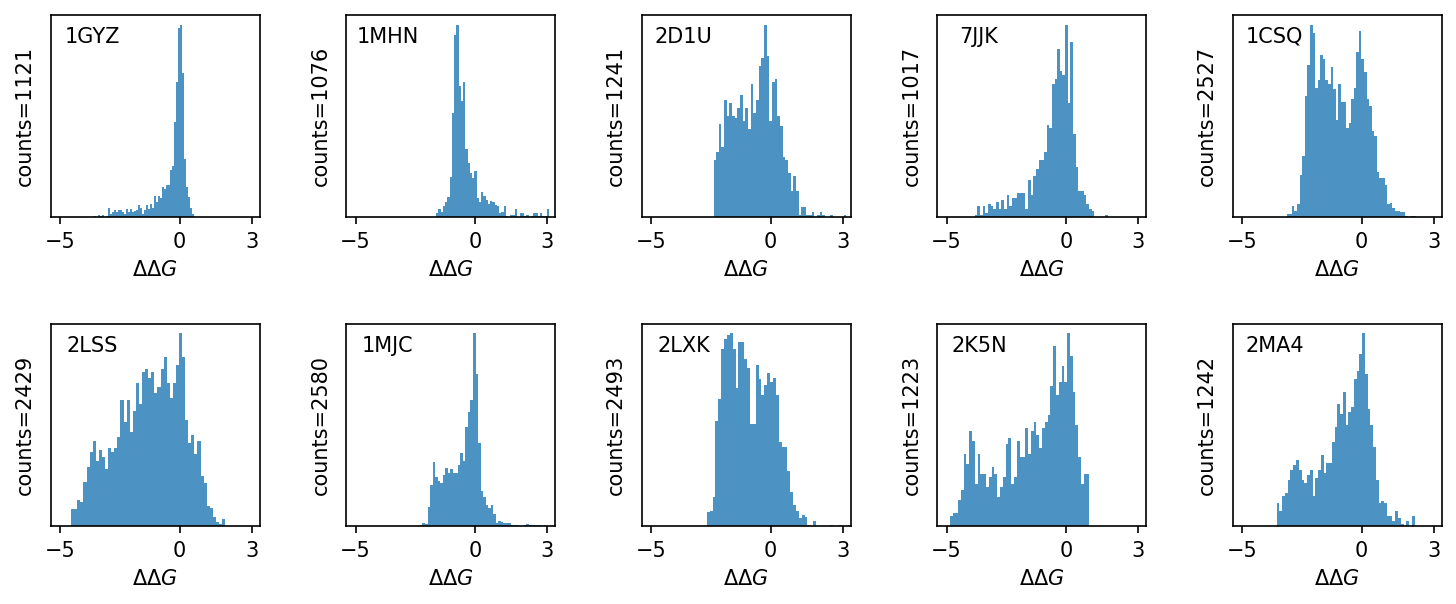
\includegraphics[width=\textwidth]{plots/wildtype.png}
    \caption{$\Delta\Delta$G histograms, for 10 wildtypes (\texttt{pdbid}). This clearly shows that \dd G is dependant on the wildtype which makes sense since it should depend on the structure.}
    \label{fig:wildtype}
\end{figure}
\FloatBarrier

\begin{figure}[!htb]
    \centering
    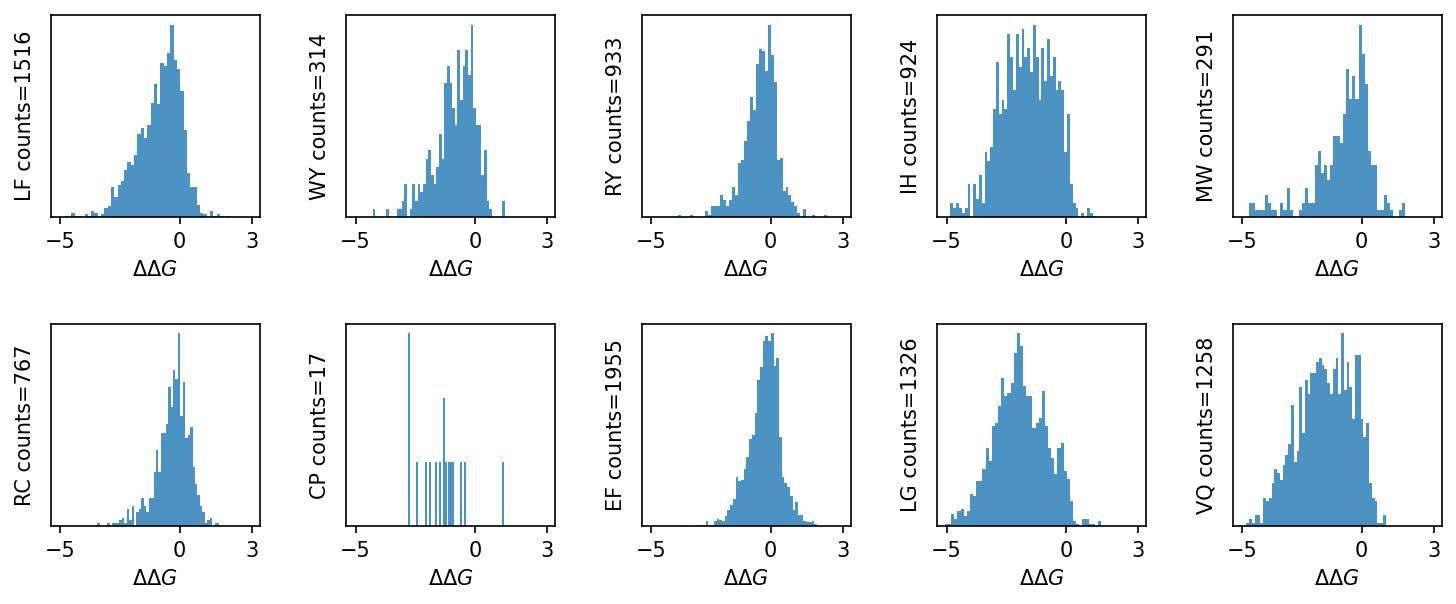
\includegraphics[width=\textwidth]{plots/mutation.png}
    \caption{$\Delta\Delta$G histograms, for 10 different mutation types (wildtype amino acid $\rightarrow$ mutant amino acid). The distributions seem to be slightly different for each mutation since the energy should depend on the amino acid substitution.}
    \label{fig:mutation}
\end{figure}
\FloatBarrier

\section{Method explanation}

\textbf{Data.} The inputs to our model should be the protein sequence itself and the mutation since these provide information for predicting $\Delta\Delta$G. To test that the models can generalize to unseen proteins, the training and test are split such that they contain completely different protein wild types (or \texttt{pdbid}). We will also use the same test set when predicting on the reverse mutations which have energy change $-\Delta\Delta$G. We've chosen a training:test split of 0.8:0.2, which is enough to train the neural network while being able to test for robustness. There are a few ways to encode the amino acids, for simplicity we will be using one-hot encodings, which is a size 20 vector of zeros (for 20 amino acids) and a 1 at the index of the amino acid, see Figure \ref{fig:lstm}. To represent the wild type to mutant amino acid transition, we also include a -1  at the index of the wild type amino acid, which is an anti-symmetric representation.
\clearpage

\begin{figure}[!htb]
    \centering
    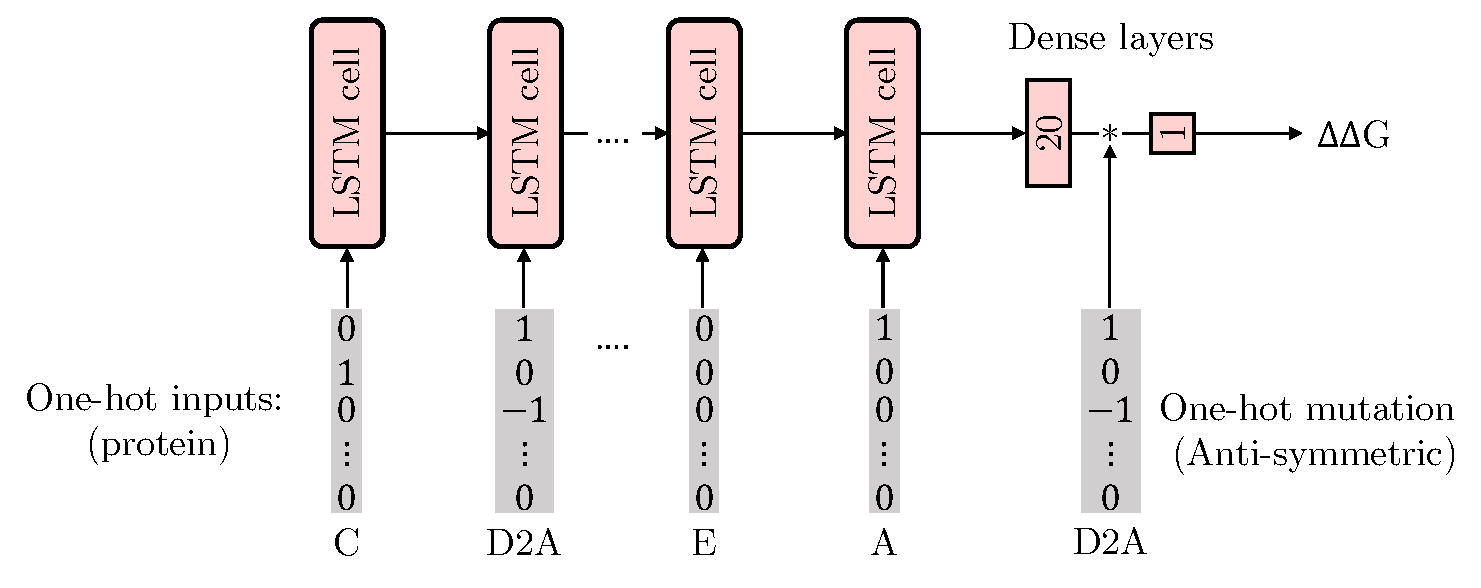
\includegraphics[width=0.8\textwidth]{lstm.pdf}
    \caption{\label{fig:lstm}LSTM model used for predicintg $\Delta\Delta$G. The inputs are one-hot encodings of the amino acid sequence, with a -1 inserted for the wild type amino acid.}
\end{figure}
\FloatBarrier

\textbf{Model.} We will be using Long Short Term Memory (LSTM) neural networks, which have been proven to work well at encoding and making predictions on sequence data. A LSTM can remember information over a wide range of intervals throughout the sequence, this is important since the protein structure (and therefore $\Delta\Delta$G) depends on short and long range electrostatic interactions. We will be using 1 recurrent LSTM cell from which the final output is applied onto 2 Dense layers which results in the final predicted $\Delta\Delta$G, see Figure \ref{fig:lstm}. To aid with anti-symmetry, we do an elementwise multiplication of the mutant amino acid with the output of the first dense layer (with no bias), i.e. $Wx = -W(-x)$, where $W$ is the weight matrix and $x$ is the one-hot mutant. We may also use anti-symmetric activation functions (e.g. tanh) and no bias on the LSTM cells to further aid anti-symmetry, but for some reason the models train a lot slower, so we ended up not doing that.

\section{Experiment description}

To correctly test our model's generalizability to unseen protein structures, the training and test datasets contain entirely different protein structures (\texttt{pdbid}). As a further generalizability test, we also predict the energy change for the test set when the wildtype (W) and mutant (M) amino acid is reversed which should give \dd G(W$\rightarrow$M)=$-$\dd G(M$\rightarrow$W).

A commonly used metric to measured the performance of models for predicting \dd G is the root mean square error (RMSE) in combination with the pearson correlation coefficient, r, which are both insufficient on their own. Together they provide a better metric to evaluate the performance for a wide range of \dd G.

\section{Result Analysis}

Figure \ref{fig:lstme}-\ref{fig:lstmae} shows the results for the (non)anti-symmetric models. We get a (RMSE, r) of (0.89, 0.48) and (0.93, 0.51). For comparison, the graph-NN from \citep{Wang2021} has (1.23, 0.61) but trained on a smaller dataset, so our model isn't that bad! But for predicting the reverse energies, Figure \ref{fig:lstmre}-\ref{fig:lstmare} shows a (RMSE, r) of (1.9, 0.1) and (1.8, 0.14), the anti-symmetric model does slightly better but they both seem to be pretty bad at generalizing to reverse energies, which is most likely due to the non-anti-symmetric LSTM cells. In comparison, \citep{Wang2021} has (1.27,0.48) for predicting reverse energies.

\begin{figure}[!htb]
    \centering
    \begin{subfigure}[b]{0.49\textwidth}
        \centering
        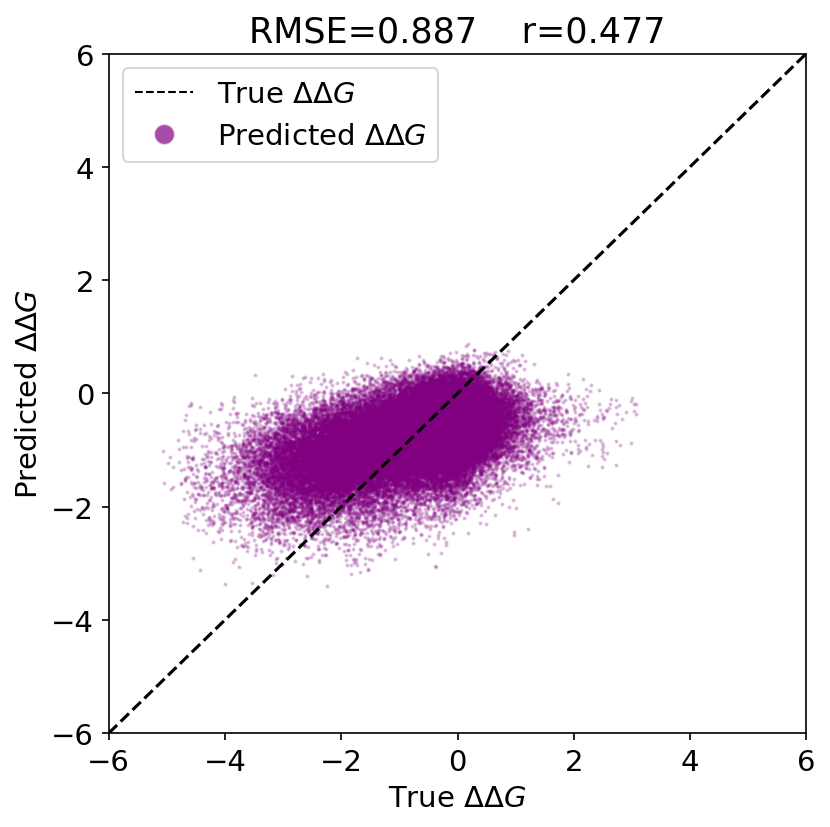
\includegraphics[width=\textwidth]{plots/lstm_error.png}
        \caption{LSTM, \dd G predictions}
        \label{fig:lstme}
    \end{subfigure}
    \hfill
    \begin{subfigure}[b]{0.49\textwidth}
        \centering
        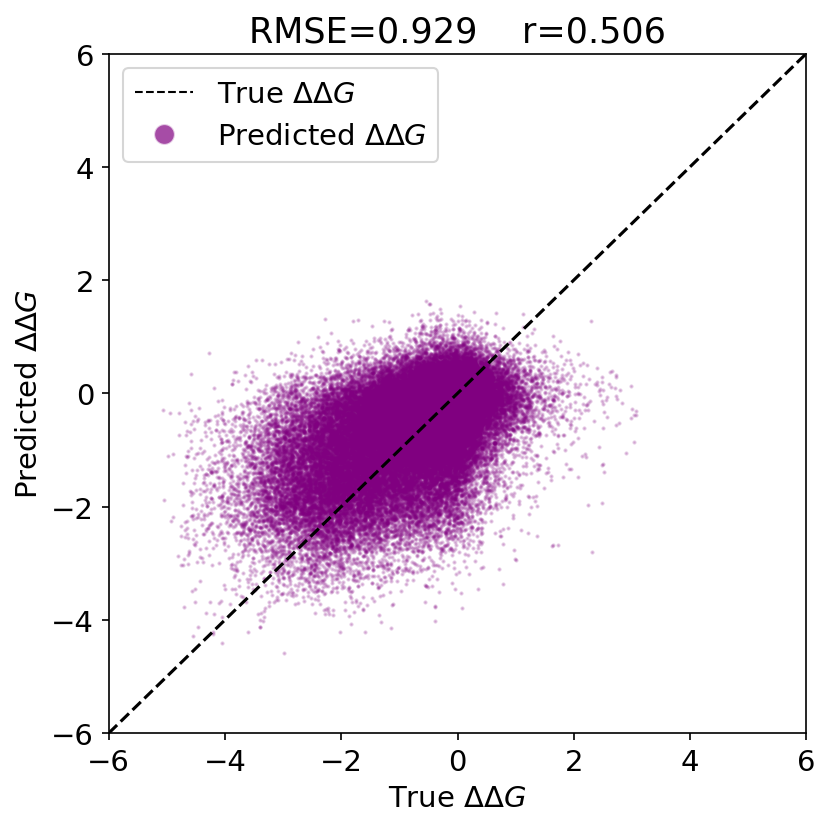
\includegraphics[width=\textwidth]{plots/lstmanti_error.png}
        \caption{anti-symmetric LSTM, \dd G predictions}
        \label{fig:lstmae}
    \end{subfigure}
    \\[3ex]
    \begin{subfigure}[b]{0.49\textwidth}
        \centering
        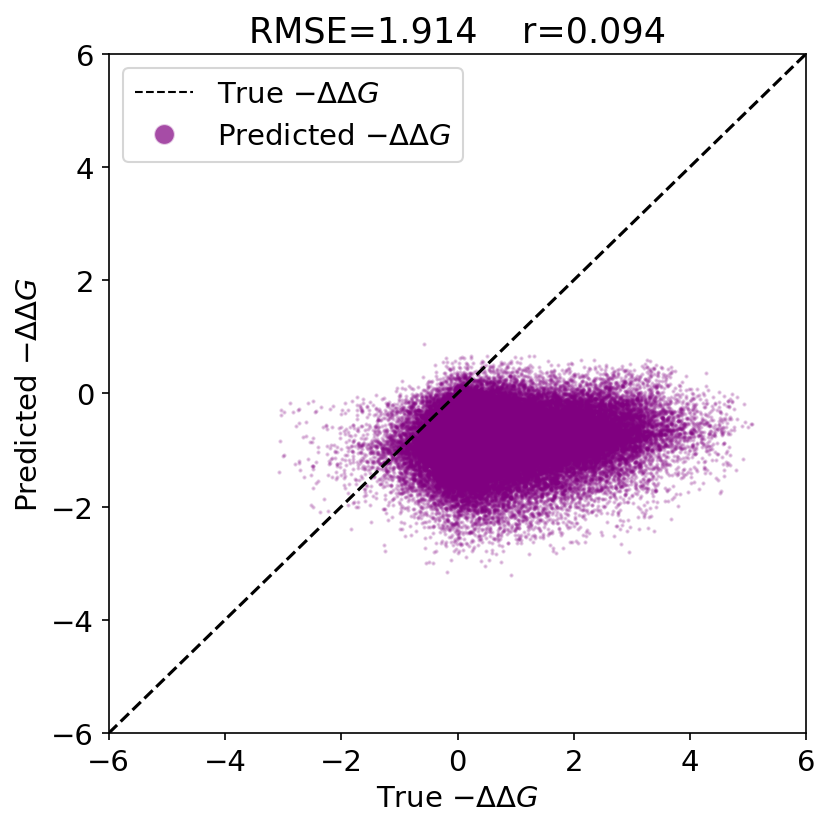
\includegraphics[width=\textwidth]{plots/lstm_error_reverse.png}
        \caption{LSTM, $-$\dd G predictions}
        \label{fig:lstmre}
    \end{subfigure}
    \hfill
    \begin{subfigure}[b]{0.49\textwidth}
        \centering
        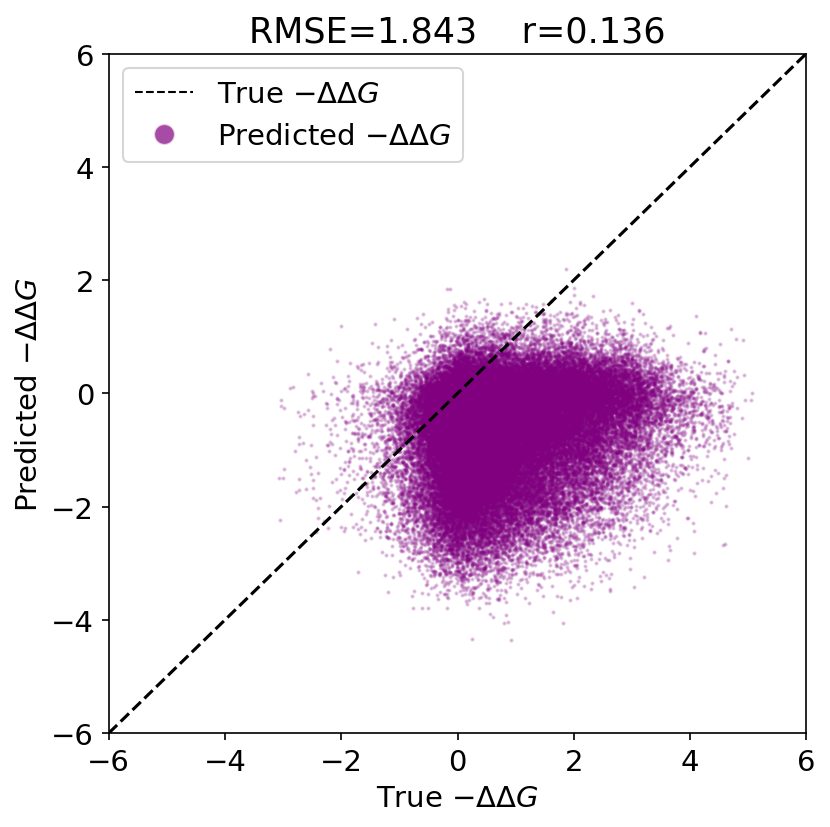
\includegraphics[width=\textwidth]{plots/lstmanti_error_reverse.png}
        \caption{anti-symmetric LSTM, $-$\dd G predictions}
        \label{fig:lstmare}
    \end{subfigure}
    \caption{True vs predicted $\pm$\dd G using the (non-)anti-symmetric LSTM models.}
    \label{fig:results}
\end{figure}
\FloatBarrier

\clearpage
\bibliography{biblio.bib}

\end{document}